\documentclass{standalone}
\usepackage{pgfplots}
\pgfplotsset{compat=1.18}
\begin{document}
\begin{tikzpicture}
  \begin{axis}[
    width=12cm,
    height=6.5cm,
    xmin=0, xmax=1.05,
    ymin=0, ymax=1.05,
    axis x line=middle, axis y line=middle,
    xlabel=$x$, ylabel=$y$,
    samples=200, domain=0:1.05,
    xtick={0,0.5,0.8333333,0.9278351,1},
    xticklabel style={font=\small},
    ytick=\empty,
    grid=none
  ]
    % functions
    \addplot[thick,black] {x}; % y = x
    \addplot[thick,orange] {5/(2*x^2+4)}; % y = 5/(2x^2+4)
    
    % compute exact points (for readability in the code)
    \pgfmathsetmacro\xzero{1}
    \pgfmathsetmacro\xone{5/6} % 0.833333...
    \pgfmathsetmacro\xtwo{90/97} % ~0.9278350515
    \pgfmathsetmacro\yone{\xone} % since point on curve at x0 is (x0, x1)
    \pgfmathsetmacro\ytwo{\xtwo} % point on line at (x2,x2)
    \pgfmathsetmacro\gofxzero{5/(2*\xzero*\xzero+4)} % g(x0) = x1
    \pgfmathsetmacro\gofxone{5/(2*\xone*\xone+4)} % g(x1) = x2

    % cobweb: start at (x0,0) up to curve (x0,x1)
    \draw[blue, thick] (axis cs:\xzero,0) -- (axis cs:\xzero,\gofxzero);
    % horizontal to line y=x at (x1,x1)
    \draw[blue, thick] (axis cs:\xzero,\gofxzero) -- (axis cs:\gofxzero,\gofxzero);
    % vertical to curve at (x1,x2)
    \draw[blue, thick] (axis cs:\gofxzero,\gofxzero) -- (axis cs:\gofxzero,\gofxone);
    % horizontal to (x2,x2)
    \draw[blue, thick] (axis cs:\gofxzero,\gofxone) -- (axis cs:\gofxone,\gofxone);
    
    % Optional: one more vertical step (shows further convergence)
    \pgfmathsetmacro\gofxtwo{5/(2*\gofxone*\gofxone+4)}
    \draw[blue, thick, dashed] (axis cs:\gofxone,\gofxone) -- (axis cs:\gofxone,\gofxtwo);
    
    % mark points on x-axis and small vertical ticks
    \draw[black] (axis cs:\xzero,0) node[below=4pt] {$x_0=1$};
    \draw[black] (axis cs:\xone,0) node[below=4pt] {$x_1=\tfrac{5}{6}\approx0.8333$};
    \draw[black] (axis cs:\xtwo,0) node[below=4pt] {$x_2=\tfrac{90}{97}\approx0.9278$};
    
    % mark the iterative points on the curves
    \filldraw[red] (axis cs:\xzero,\gofxzero) circle (1.6pt) node[above right, inner sep=1pt] {$ x_0,x_1$};
    \filldraw[red] (axis cs:\gofxzero,\gofxone) circle (1.6pt) node[above right, inner sep=1pt] {$ x_1,x_2$};
    \filldraw[red] (axis cs:\gofxone,\gofxone) circle (1pt); % (x2,x2) point on y=x
    
    % legend-like labels
    \node[black, right] at (axis cs:0.3,0.95) {$y=x$};
    \node[orange, right] at (axis cs:0.7,0.65) {$y=\frac{5}{2x^{2}+4}$};
    \node[blue, right] at (axis cs:0.35,0.75) {Cobweb iterations};
  \end{axis}
\end{tikzpicture}
\end{document}